% Drawing 154/08-20 -- folder 154, batch 08, archive page 146 (PDF page 147).
% Transcription: cinq disques au crayon et à l'encre, sans texte : un disque traversé de pseudo-droites qui se croisent ; un cercle vide ; un disque dont deux points opposés du bord sont joints par un faisceau dense de courbes brunes ; un disque traversé de courbes enchevêtrées ; un disque traversé de quelques droites entre deux points marqués du bord
% Kind: five pencil disks. Method 2 (schematic redraw from the facsimile). Status: partial.
% Notes: Five circles placed as on the page (the transcription's note says « quatre disques » and then lists five). Upper left: a disk with five strands. Middle: an empty oval, very faint. Lower left: a disk whose top and bottom points are joined by a dense sheaf of brown curves, of which seven are drawn. Lower middle: a disk with tangled curves, of which six are drawn, a point at the bottom of its rim. Lower right: a disk with a marked point at the top and one below the rim at the bottom, joined by a straight stroke, and three other chords. In every disk the strands are indicative: their number and their crossings are not those of the page. Redrawn 2026-11-12 (issue 128): to check again. 2026-11-14, Claude Opus 5.5, overlay check (issue 147): rasterised from its own coordinates over the 400 dpi colour scan (402 ppi native) on a unit grid; not compiled (no TeX in the session). The rims of the five pencil disks, the oval and the marked points lie on their ink to within about 1 unit; the redraw is unchanged. Still partial, as said above: the strands inside the disks are indicative and do not lie on their pencil (in places 2 to 5 units off); they would have to be traced one by one.
% Coordinates: 1 unit = 1 mm = 1/100 of the crop width (bbox in page fractions: [0.115, 0.185, 0.8, 0.53]).
% Redrawn by Claude (claude-fable-5-2), issue #128, 2026-11-12; not checked by a human; not compiled (no TeX in the session).
% Checked by Claude (claude-opus-5-5) 2026-11-14 (issue #147): overlaid on the 400 dpi colour facsimile; not compiled (no TeX in the session). Not checked by a human. Status: partial.
% Rights: reproduces part of the work -- behind RENDER_TRANSCRIPTS, never published by itself.
\documentclass[tikz,border=3pt]{standalone}
\usepackage{amsmath,amssymb}
\usetikzlibrary{patterns,arrows.meta}
\tikzset{Br/.style={brown!80!black}, pencil/.style={black!45}, struck/.style={black!35}, mpt/.style={circle,draw,inner sep=1.3pt}, pt/.style={circle,fill,inner sep=0.9pt}, opt/.style={circle,draw,fill=white,inner sep=1.1pt}}
\begin{document}
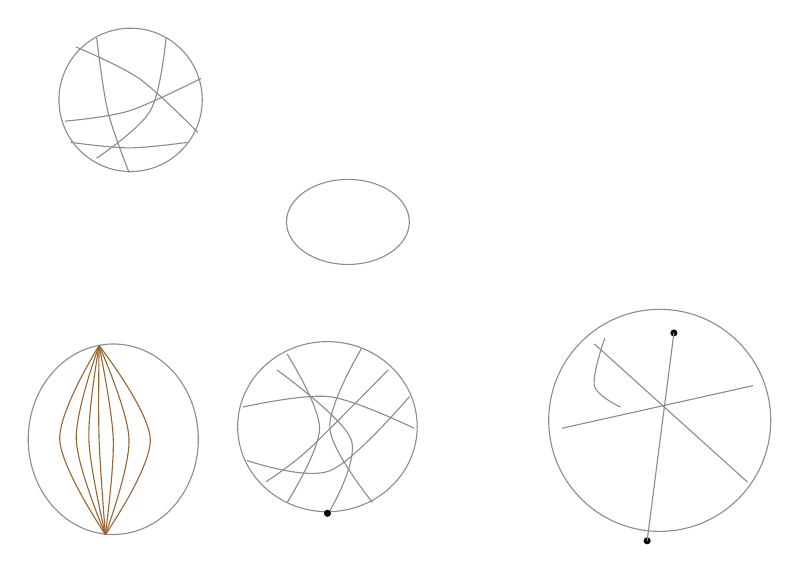
\begin{tikzpicture}[x=1mm,y=1mm,line cap=round,line join=round,font=\scriptsize]
\draw[pencil] (16,-13.2) circle[radius=9.1];
\draw[pencil] plot[smooth, tension=0.55] coordinates {(11.7,-5.4) (13.1,-14.6) (15.8,-22.4)};
\draw[pencil] plot[smooth, tension=0.55] coordinates {(9.1,-6.5) (17.1,-10.5) (24.5,-17.3)};
\draw[pencil] plot[smooth, tension=0.55] coordinates {(7.7,-15.9) (15.8,-14.6) (24.9,-10.5)};
\draw[pencil] plot[smooth, tension=0.55] coordinates {(20.5,-5.4) (18.5,-14.6) (11.7,-20.6)};
\draw[pencil] plot[smooth, tension=0.55] coordinates {(8.4,-18.6) (15.8,-19.3) (23.2,-18.6)};
\draw[pencil] (43.6,-28.7) ellipse[x radius=7.8, y radius=5.4];
\draw[pencil] (13.8,-56.3) ellipse[x radius=10.8, y radius=12.1];
\draw[Br] plot[smooth, tension=0.55] coordinates {(12,-44.4) (7,-56.3) (12.8,-68.4)};
\draw[Br] plot[smooth, tension=0.55] coordinates {(12,-44.4) (9.1,-56.3) (12.8,-68.4)};
\draw[Br] plot[smooth, tension=0.55] coordinates {(12,-44.4) (10.7,-56.3) (12.8,-68.4)};
\draw[Br] plot[smooth, tension=0.55] coordinates {(12,-44.4) (12,-56.3) (12.8,-68.4)};
\draw[Br] plot[smooth, tension=0.55] coordinates {(12,-44.4) (13.8,-56.3) (12.8,-68.4)};
\draw[Br] plot[smooth, tension=0.55] coordinates {(12,-44.4) (15.8,-56.3) (12.8,-68.4)};
\draw[Br] plot[smooth, tension=0.55] coordinates {(12,-44.4) (18.5,-56.3) (12.8,-68.4)};
\draw[pencil] (41,-54.7) ellipse[x radius=11.4, y radius=10.8];
\draw[pencil] plot[smooth, tension=0.55] coordinates {(35.9,-45.5) (40,-54.9) (35.9,-64.3)};
\draw[pencil] plot[smooth, tension=0.55] coordinates {(45.3,-44.8) (41.3,-54.9) (46.7,-64.3)};
\draw[pencil] plot[smooth, tension=0.55] coordinates {(30.3,-52.2) (41.3,-50.9) (52,-54.9)};
\draw[pencil] plot[smooth, tension=0.55] coordinates {(30.8,-59) (41.3,-60.3) (51.4,-50.9)};
\draw[pencil] plot[smooth, tension=0.55] coordinates {(34.6,-47.5) (44,-56.3) (41.3,-65.4)};
\draw[pencil] plot[smooth, tension=0.55] coordinates {(48.7,-47.5) (38.6,-57.6) (33.2,-61.7)};
\node[pt] at (41,-65.7) {};
\draw[pencil] (83.2,-53.9) circle[radius=14.1];
\node[pt] at (85,-42.8) {};
\node[pt] at (81.6,-69.2) {};
\draw[pencil] (85,-42.8) -- (81.6,-69.2);
\draw[pencil] (70.8,-54.9) -- (95,-49.5);
\draw[pencil] (74.9,-44.2) -- (94.3,-61.7);
\draw[pencil] plot[smooth, tension=0.55] coordinates {(76.2,-43.5) (74.9,-49.5) (78.2,-52.2)};
\end{tikzpicture}
\end{document}
